% $Header$
% MBDyn (C) is a multibody analysis code.
% http://www.mbdyn.org
%
% Copyright (C) 1996-2017
%
% Pierangelo Masarati  <masarati@aero.polimi.it>
%
% Dipartimento di Ingegneria Aerospaziale - Politecnico di Milano
% via La Masa, 34 - 20156 Milano, Italy
% http://www.aero.polimi.it
%
% Changing this copyright notice is forbidden.
%
% This program is free software; you can redistribute it and/or modify
% it under the terms of the GNU General Public License as published by
% the Free Software Foundation (version 2 of the License).
% 
%
% This program is distributed in the hope that it will be useful,
% but WITHOUT ANY WARRANTY; without even the implied warranty of
% MERCHANTABILITY or FITNESS FOR A PARTICULAR PURPOSE.  See the
% GNU General Public License for more details.
%
% You should have received a copy of the GNU General Public License
% along with this program; if not, write to the Free Software
% Foundation, Inc., 59 Temple Place, Suite 330, Boston, MA  02111-1307  USA

\chapter{Problems}\label{sec:PROBLEMS}
This section is used to insert all the data related to the problem that
one needs MBDyn to solve in the simulation.
The section data are included between the cards:
%\begin{verbatim}
\begin{Verbatim}[commandchars=\\\{\}]
    \kw{begin} : \bnt{problem_name} ;
        # ...
    \kw{end} : \bnt{problem_name} ;
\end{Verbatim}
%\end{verbatim}

Implemented problems are:
\begin{itemize}
\item \kw{initial value}, the time integration of mechanical
and multidisciplinary problems formulated
as Differential-Algebraic Equations (DAE).
It can be downgraded to the solution of static and kinematic problems,
by selecting purely static or kinematic contributions
to the governing equations, thus giving time the role
of an ordinal parameter.

\item \kw{inverse dynamics}, the computation of the generalized forces
required to make a generic system perform a given trajectory.

\end{itemize}





\section{Initial-Value Problem}
\label{sec:IVP}
At present, the main problem is \kw{initial value},
which solves initial value problems
by means of generic integration schemes that can be cast
in a broad family of multistep and, experimentally,
Implicit Runge-Kutta-like schemes
\cite{MASARATI-LANZ-MANTEGAZZA-2001}.

The syntax of the module is:
%\begin{verbatim}
\begin{Verbatim}[commandchars=\\\{\}]
    \kw{begin} : \kw{initial value} ;
        # ...
    \kw{end} : \kw{initial value} ;
\end{Verbatim}
%\end{verbatim}
At present, there are a number of cards that can be grouped as follows, 
based on the integration phase they refer to.

\subsection{General Data}
those data that refer to the main integration phase or the simulation as a
whole. They are:

\subsubsection{Initial Time}
%\begin{verbatim}
\begin{Verbatim}[commandchars=\\\{\}]
    \bnt{card} ::= \kw{initial time} : \bnt{time} ;
\end{Verbatim}
%\end{verbatim}

\subsubsection{Final Time}
%\begin{verbatim}
\begin{Verbatim}[commandchars=\\\{\}]
    \bnt{card} ::= \kw{final time} : \{ \kw{forever} | \bnt{time} \} ;
\end{Verbatim}
%\end{verbatim}

\subsubsection{Strategy}
%\begin{verbatim}
\begin{Verbatim}[commandchars=\\\{\}]
    \bnt{card} ::= \kw{strategy} : \bnt{strategy_type} [ , \bnt{strategy_data} ] ;
\end{Verbatim}
%\end{verbatim}
The available strategies are:
\begin{itemize}
\item \kw{no change}
%\begin{verbatim}
\begin{Verbatim}[commandchars=\\\{\}]
    \bnt{strategy_type} ::= \kw{no change}
\end{Verbatim}
%\end{verbatim}
the time step is never changed.
However, this prevents simulation termination when the maximum number
of iterations is reached.
As a consequence, its use only makes sense when repeating a time step
results in some modification of the analysis related to some user-defined
function.

\item \kw{factor}
%\begin{verbatim}
\begin{Verbatim}[commandchars=\\\{\}]
    \bnt{strategy_type} ::= \kw{factor}

    \bnt{strategy_data} ::= 
        \bnt{reduction_factor} ,
        \bnt{steps_before_reduction} ,
        \bnt{raise_factor} ,
        \bnt{steps_before_raise} ,
        \bnt{min_iterations}
        [ , \bnt{max_iterations} ]
\end{Verbatim}
%\end{verbatim}
the time step is reduced or raised of the proper factor not before a
minimum number of time steps; it is reduced if more than 
\nt{max\_iterations} are performed at a time step, or it the current
step do not converge; it is raised if less
than \nt{min\_iterations} are performed at a time step;
\nt{max\_iterations} defaults to the global \nt{max\_iterations}
simulation value; however, it is better to set it to a lower value,
leaving some spare iterations before bailing out the simulation; 
the simulation bails out if two consecutive solution steps
are performed without converging.

\item \kw{change}
%\begin{verbatim}
\begin{Verbatim}[commandchars=\\\{\}]
    \bnt{strategy_type} ::= \kw{change}

    \bnt{strategy_data} ::= (\hty{DriveCaller}) \bnt{time_step_pattern}
\end{Verbatim}
%\end{verbatim}
the time step is changed according to the \nt{time\_step\_pattern} pattern.
If the time step returned by the drive caller does not change
when a step needs to be repeated, the analysis is interrupted.

Note: the \kw{change} strategy is not normally intended to provide
adaptive time step, it rather allows to prescribe a given
variable time step pattern based on the rule defined
by the \nt{time\_step\_pattern} \hty{DriveCaller}.
\end{itemize}
In any case, step change only occurs after the first step, which is performed
using the \nt{time\_step} value provided with the \kw{time step} statement.


\subsubsection{Min Time Step}
%\begin{verbatim}
\begin{Verbatim}[commandchars=\\\{\}]
    \bnt{card} ::= \kw{min time step} : \bnt{min_time_step} ;
\end{Verbatim}
%\end{verbatim}
Defines the minimum value allowed for the time step.
This statement is only meaningful when variable time step is used.
If the time step change strategy tries to use a time step smaller
than \nt{min\_time\_step}, the simulation aborts.

\subsubsection{Max Time Step}
%\begin{verbatim}
\begin{Verbatim}[commandchars=\\\{\}]
    \bnt{card} ::= \kw{max time step} : \{ \bnt{max_time_step} | \kw{unlimited} \} ;
\end{Verbatim}
%\end{verbatim}
Defines the maximum value allowed for the time step.
This statement is only meaningful when variable time step is used.
If the time step change strategy tries to use a time step larger
than \nt{max\_time\_step}, the value \nt{max\_time\_step} is used instead.

\subsubsection{Time Step}
%\begin{verbatim}
\begin{Verbatim}[commandchars=\\\{\}]
    \bnt{card} ::= \kw{time step} : \bnt{time_step} ;
\end{Verbatim}
%\end{verbatim}
The initial time step.
This value is used throughout the simulation unless some variable time step
strategy is defined using the \kw{strategy} statement.

\subsubsection{Tolerance}\label{sec:IVP:TOLERANCE}
%\begin{verbatim}
\begin{Verbatim}[commandchars=\\\{\}]
    \bnt{card} ::= \kw{tolerance} : \{ \kw{null} | \bnt{residual_tolerance} \}
            [ , \kw{test} , \{ \kw{none} | \kw{norm} | \kw{minmax} \} [ , \kw{scale} ] ]
        [ , \{ \kw{null} | \bnt{solution_tolerance} \} 
            [ , \kw{test} , \{ \kw{none} | \kw{norm} | \kw{minmax} \} ] ] ;
\end{Verbatim}
%\end{verbatim}
The only mandatory value is \nt{residual\_tolerance}, 
the tolerance used for the residual test; the keyword \kw{null}
disables the residual testing, disabling the computation
of the test on the residual.
The \kw{test} mechanism is used to select what kind of test must
be performed; currently, only \kw{norm} (the default) 
and \kw{minmax} are supported.
The special value \kw{none} means that the test is not actually 
computed; it is the default when the test is disabled by setting
the tolerance to zero, or by using the keyword \kw{null};
however, it can be restored to any mechanism for output purposes.
The optional parameter \kw{scale} is used to enable the scaling
of the residual before performing the test; default scale factors 
can be set for each type of degree of freedom owner, as seen for the control data item of Section~\ref{sec:CONTROLDATA:DEFAULTSCALE}; some
entities allow individual scaling, as seen for nodes in Chapter~\ref{sec:NODES}; by default, no scaling takes place.
A tolerance \nt{solution\_tolerance} to test the solution 
(the difference between the states at two iterations) is allowed, 
and also in this case a test mechanism can be chosen;
by default, no test on the solution convergence is done.
Currently, no scaling is allowed in the solution test.

\noindent
\paragraph{Example.} \
\begin{verbatim}
    # residual test by means of the norm
    tolerance: 1.e-6;
    # residual test with minmax method
    tolerance: 1.e-6, test, minmax;
    # residual test with norm method and scaling
    tolerance: 1.e-6, test, norm, scale;
    # solution test
    tolerance: null, 1.e-9;
    # residual and solution test
    # (the first that succeeds breaks the loop)
    tolerance: 1.e-6, 1.e-9;
    # residual test with computation of solution norm
    tolerance: 1.e-6, null, test, norm;
\end{verbatim}

\subsubsection{Max Iterations}
%\begin{verbatim}
\begin{Verbatim}[commandchars=\\\{\}]
    \bnt{card} ::= \kw{max iterations} : \bnt{max_iterations} [ , \kw{at most} ] ;
\end{Verbatim}
%\end{verbatim}
Error out after \nt{max\_iterations} without passing the convergence test.
The default value is zero.

If the optional keywords \kw{at most} are given,
the step is considered successfully performed after \nt{max\_iterations}
regardless of passing the convergence test, as soon as the error
reduced since the first iteration.
For example, when using
\begin{verbatim}
    max iterations: 5, at most;
\end{verbatim}
the convergence pattern
\begin{verbatim}
    ...
        Iteration(0) 1.16374e+06 J
                SolErr 0
        Iteration(1) 8330.76 J
                SolErr 0
        Iteration(2) 43768.8 J
                SolErr 0
        Iteration(3) 2981.01 J
                SolErr 0
        Iteration(4) 118839 J
                SolErr 0
        Iteration(5) 8654.02 J
    ...
\end{verbatim}
succeeds, since $8654.02 < 1.16374\text{e$+$}06$, while
\begin{verbatim}
    ...
        Iteration(0) 1.66901e+06 J
                SolErr 0
        Iteration(1) 2.06327e+09 J
                SolErr 0
        Iteration(2) 2.64337e+10 J
                SolErr 0
        Iteration(3) 1.2131e+12 J
                SolErr 0
        Iteration(4) 7.08449e+12 J
                SolErr 0
        Iteration(5) 2.18828e+15 J
Max iterations number 5 has been reached during Step=6, Time=0.06; \
TimeStep=0.01 cannot be reduced further; aborting...
An error occurred during the execution of MBDyn; aborting... 
\end{verbatim}
fails since $2.18828\text{e$+$}15 > 1.66901\text{e$+$}06$.

\fbox{\textbf{This option should be used with extreme care.}}

\subsubsection{Modify Residual Test}
%\begin{verbatim}
\begin{Verbatim}[commandchars=\\\{\}]
    \bnt{card} ::= \kw{modify residual test} ;
\end{Verbatim}
%\end{verbatim}
modify the residual test taking in account the rate of change of the status.

\subsubsection{Method}
%\begin{verbatim}
\begin{Verbatim}[commandchars=\\\{\}]
    \bnt{card} ::= \kw{method} : \bnt{method_data} ;
\end{Verbatim}
%\end{verbatim}
there are four multistep methods at present. 

The first is Crank-Nicolson:
%\begin{verbatim}
\begin{Verbatim}[commandchars=\\\{\}]
    \bnt{method_data} ::= \kw{crank nicolson}
\end{Verbatim}
%\end{verbatim}

The second and the third are original 
methods; the former is discussed in \cite{MASARATI-LANZ-MANTEGAZZA-2001},
see also
\begin{quote}
\htmladdnormallink{\texttt{http://www.aero.polimi.it/mbdyn/publications.html}}{http://www.aero.polimi.it/mbdyn/publications.html}
\end{quote} 
Those methods are unconditionally stable and can be tuned to give 
the desired algorithmic dissipation
by setting the value of the asymptotic spectral radius.
The radius can be set independently for the differential
and the algebraic variables, and a driver is used, to allow parameter 
dependent radius variation.
%\begin{verbatim}
\begin{Verbatim}[commandchars=\\\{\}]
    \bnt{method_data} ::= \{ \kw{ms} | \kw{hope} \} ,
        (\hty{DriveCaller}) \bnt{differential_radius}
        [ , (\hty{DriveCaller}) \bnt{algebraic_radius} ]
\end{Verbatim}
%\end{verbatim}
The first method proved to be more accurate at high values of asymptotic
radius (low dissipation), while the second proved to be more accurate
at low values of the radius (high dissipation).
They look nearly equivalent at radii close to 0.4, with the former
giving the best compromise between algorithmic dissipation and accuracy 
at about 0.6.
The \nt{algebraic\_radius} can be omitted, defaulting to the same 
as the differential one.
It is unclear whether a different spectral radius can help in increasing
accuracy or dissipation of the algebraic unknowns.

The fourth method is experimental. It is a third-order,
two stage unconditionally stable method, which can be tuned to give 
the desired algorithmic dissipation by setting the value 
of the asymptotic spectral radius, which should not be 
too close to zero.
Currently it is not possible to independently set the radius 
for the differential and the algebraic variables.
%\begin{verbatim}
\begin{Verbatim}[commandchars=\\\{\}]
    \bnt{method_data} ::= \kw{third order} ,
        \{ \kw{ad hoc} | (\hty{DriveCaller}) \bnt{differential_radius} \}
\end{Verbatim}
%\end{verbatim}
When the keyword \kw{ad hoc} is used, a method equivalent
to a Runge-Kutta Radau IIA results, with zero asymptotic
spectral radius; otherwise, an original third-order
integration method is used, with tunable algorithmic dissipation.

\noindent
The multistep method, when the asymptotic radius is zero, degenerates
in the Backward Differentiation Formulas of order two.
A shortcut to this case is provided as
%\begin{verbatim}
\begin{Verbatim}[commandchars=\\\{\}]
    \bnt{method_data} ::= \kw{bdf} [ , \kw{order} , \bnt{order} ]
\end{Verbatim}
%\end{verbatim}
The keyword \kw{order} can be used to indicate a specific \nt{order}
of the Backward Differentiation Formulas (BDF); only first order (implicit Euler) and 
second order formulas are currently implemented, and the default
is the second order formula, which is the most useful.
The first order formula may be of help for very specific problems.
It can also be selected using the shortcut
%\begin{verbatim}
\begin{Verbatim}[commandchars=\\\{\}]
    \bnt{method_data} ::= \kw{implicit euler}
\end{Verbatim}
%\end{verbatim}

\subsubsection{Nonlinear Solver}
The nonlinear solver solves a nonlinear problem $F(x)=0$.
The syntax is
%\begin{verbatim}
\begin{Verbatim}[commandchars=\\\{\}]
    \bnt{card} ::= \kw{nonlinear solver} : \bnt{nonlinear_solver_name}
        [ , \bnt{nonlinear_solver_data} ] ;
\end{Verbatim}
%\end{verbatim}
Currently available nonlinear solvers are:

\paragraph{Newton-Raphson.}
%\begin{verbatim}
\begin{Verbatim}[commandchars=\\\{\}]
    \bnt{nonlinear_solver_name} ::= \kw{newton raphson}

    \bnt{nonlinear_solver_data} ::=
        [ \{ \kw{true}
        | \kw{modified} , \bnt{iterations}
            [ , \kw{keep jacobian matrix} ]
            [ , \kw{honor element requests} ] \} ] ;
\end{Verbatim}
%\end{verbatim}
if \kw{modified}, the number of \nt{iterations} the same Jacobian matrix 
will be reused, and thus factored only once, is expected.
If the option \kw{keep jacobian matrix} is selected,
the Jacobian matrix is preserved
for the desired \nt{iterations} even across time steps.
By default, the Jacobian matrix is recomputed at the beginning 
of each time step.
If the option \kw{honor element requests} is selected, the factorization
is updated also when an element changes the structure of its equations.
The default behavior is to ignore such requests\footnote{
	At present, only few elements that can change the structure
	of the equations, or at least radically change the Jacobian matrix,
	actually issue this request.
}.
This nonlinear solver is well tested.

\paragraph{Line search.}
\emph{Author: Reinhard Resch}
\begin{Verbatim}[commandchars=\\\{\}]
    \bnt{nonlinear_solver_name} ::= \kw{line search | bfgs}

    \bnt{nonlinear_solver_data} ::= 
        [ \{ \kw{true}
        | \kw{modified} , \bnt{iterations}
            [ , \kw{keep jacobian matrix} ]
            [ , \kw{honor element requests} ] \} ]
        [ , \kw{tolerance x} , \bnt{tolerance_x} ]
        [ , \kw{tolerance min} , \bnt{tolerance_min} ]
        [ , \kw{max iterations} , \bnt{max_iterations} ]
        [ , \kw{alpha} , \bnt{alpha} ]
        [ , \kw{lambda min} , \bnt{lambda_min}
            [ , \kw{relative} , \{ \kw{yes} | \kw{no} | (\ty{bool}) \bnt{relative} \} ] ]
        [ , \kw{lambda factor min} , \bnt{lambda_factor_min} ]
        [ , \kw{max step} , \bnt{max_step} ]
        [ , \kw{zero gradient} , \kw{continue} , \{ \kw{yes} | \kw{no} | (\ty{bool}) \bnt{zero_gradient_continue} \} ]
        [ , \kw{divergence check} , \{ \kw{yes} | \kw{no} | (\ty{bool}) \bnt{divergence_check} \}
            [ , \kw{factor} , \bnt{factor} ] ]
        [ , \kw{algorithm} , \{ \kw{cubic} | \kw{factor} \} ]
        [ , \kw{scale newton step} , \{ \kw{yes} | \kw{no} | (\ty{bool}) \bnt{scale\_newton\_step} \}
            [ , \kw{min scale} , \bnt{min_scale} ] ]
        [ , \kw{print convergence info} , \{ \kw{yes} | \kw{no} | (\ty{bool}) \bnt{print_convergence_info} \} ]
        [ , \kw{verbose} , \{ \kw{yes} | \kw{no} | (\ty{bool}) \bnt{verbose} \} ]
        [ , \kw{abort at lambda min} , \{ \kw{yes} | \kw{no} | (\ty{bool}) \bnt{abort_at_lambda_min} \} ] ;
\end{Verbatim}
\begin{itemize}
\item $\nt{tolerance\_x} \ge 0$; default: $\nt{tolerance\_x}=10^{-7}$
\item $\nt{tolerance\_min} \ge 0$; default: $\nt{tolerance\_min} = 10^{-8}$
\item $\nt{max\_iterations} \ge 0$; default: $\nt{max\_iterations} = 200$
\item $\nt{alpha} \ge 0$; default: $\nt{alpha}=10^{-4}$
\item $\nt{lambda\_min} \ge 0$; default: $\nt{lambda\_min}=10^{-2}$
\item $0 < \nt{lambda\_factor\_min} < 1$; default: $\nt{lambda\_factor\_min}=10^{-1}$
\item $\nt{max\_step} \ge 0$; default: $\nt{max\_step} = 100$
\item $\nt{factor} \ge 0$; default: $\nt{factor} = 1$
\item $0 \le \nt{min\_scale} \le 1$; default: $\nt{min\_scale}=10^{-3}$
\end{itemize}

\subparagraph{Brief description of the solver}
The line search solver should be used mainly if the Newton Raphson solver diverges and further reduction of the time step is not possible or not available. In many situations this solver is able to handle larger time steps or load increments than the ordinary Newton Raphson solver. However the total number of iterations can increase for large time steps.

\subparagraph{The ordinary Newton Raphson strategy}
The Newton Raphson Solver solves a problem of the form $\boldsymbol{F}\left(\boldsymbol{x}\right)=\boldsymbol{0}$ by means of the iteration $\delta\boldsymbol{x}=\boldsymbol{J}^{-1}\,\boldsymbol{F}$.

\begin{description}
\item[$\delta\boldsymbol{x}$] The increment of the solution $\boldsymbol{x}$ during one iteration.
\item[$\boldsymbol{J}$] The modified Jacobian matrix. 
For example during the initial assembly phase $\boldsymbol{J}=-\frac{\partial \boldsymbol{F}}{\partial \boldsymbol{x}}$. 
On the other hand during the regular solution phase of an initial value problem $\boldsymbol{J}=-\frac{\partial \boldsymbol{F}}{\partial \dot{\boldsymbol{x}}}-c\,\frac{\partial \boldsymbol{F}}{\partial \boldsymbol{x}}$
and $\delta\dot{\boldsymbol{x}}=\boldsymbol{J}^{-1}\,\boldsymbol{F}$ whereas $\delta\boldsymbol{x}=c\,\delta\dot{\boldsymbol{x}}$. But that's totally transparent to the nonlinear solver.
\end{description}

If the prediction for $\boldsymbol{x}$ is close enough to the solution of the problem, the convergence rate will be quadratic as long as $\boldsymbol{J}$ is exact and $\boldsymbol{F}$ is continuously differentiable in the neighborhood of $\boldsymbol{x}$. Otherwise the rate of convergence will be not as good or even worse, the solution could diverge. The standard way to overcome such problems is to reduce the time step or to use adaptive time step control. If there are still convergence problems, the line search solver can be used.

\subparagraph{The basic idea of line search}
The line search solver from \cite{NUMERICAL-RECIPES-IN-C} uses the following modified strategy:

\begin{equation}
\delta\boldsymbol{x}=\lambda\,\boldsymbol{J}^{-1}\,\boldsymbol{F}
\end{equation}

\begin{description}
\item[$0 < \lambda \le 1$] a scalar parameter
\end{description}

In other words the direction of the increment $\delta\boldsymbol{x}$ is the same like with the Newton Raphson solver but the step size can be optionally reduced by the factor $\lambda$ in order to avoid divergence.

\subparagraph{How to determine $\lambda$}
The parameter $\lambda$ is chosen by the algorithm at each iteration in order to minimize the scalar function $f=\frac{1}{2}\,\boldsymbol{F}^T\,\boldsymbol{F}$ during the line search along the Newton direction $\delta\boldsymbol{x}$. Since the Newton direction $\delta\boldsymbol{x}$ is a descent direction for $f$, it is guaranteed that the residual will decrease at each iteration as long as $\nabla f \neq \boldsymbol{0}$, $\boldsymbol{J}$ is exact and $\boldsymbol{F}\left(\boldsymbol{x}\right)$ is continuously differentiable in the neighborhood of $\boldsymbol{x}$.

\subparagraph{Local minimum}
However it could happen that the solver converges to a local minimum of $f$ where $\nabla f = \boldsymbol{0}$ but $\boldsymbol{F} \neq \boldsymbol{0}$.
The default behavior of the solver is to bail out in such a situation unless \kw{zero gradient}, \kw{continue}, \kw{yes} has been specified. This flag has been added in order to test the solver but should not be used in general. If the solver bails out because the gradient $\nabla f$ is close to zero, it is recommended to decrease either $\bnt{tolerance\_min}$ or to reduce the time step.

\subparagraph{Cubic interpolation of $f\left(\lambda\right)$}
Two different strategies in order to determine $\lambda$ have been implemented.
The original one published in \cite{NUMERICAL-RECIPES-IN-C} which uses a cubic interpolation of $f\left(\lambda\right)$ will be used if \kw{algorithm}, \kw{cubic} was specified in the input file.
In order to avoid too small increments $\delta\boldsymbol{x}$, a value for $\nt{lambda\_factor\_min}$ can be specified.

\begin{equation}
\lambda_{n+1} \geq \nt{lambda\_factor\_min} \, \lambda_{n}
\end{equation}

\subparagraph{Multiplication by a constant factor}
Also a simple algorithm, which multiplies $\lambda$ by the constant factor $\nt{lambda\_factor\_min}$ at each line search iteration, can be used if \kw{algorithm}, \kw{factor} is specified in the input file.

\subparagraph{The condition for backtracking}
According to \cite{NUMERICAL-RECIPES-IN-C} the line search is completed if

\begin{eqnarray}
f &<& f_{prev} + \nt{alpha} \, s \\ \nonumber
\end{eqnarray}

\begin{description}
\item[$s=\left(\nabla f\right)^T\,\boldsymbol{J}^{-1}\,\boldsymbol{F} = -\boldsymbol{F}^T\,\boldsymbol{F} < 0$]:
the initial slope of decrease of $f$ is the projection of the gradient $\nabla f$ to the Newton direction $\delta\boldsymbol{x}$.
\item[$\nabla f=-\boldsymbol{J}^T\,\boldsymbol{F}$]: the gradient of $f$
\item[$f_{prev}$]: the value of $f$ at the previous iteration
\end{description}

\subparagraph{If line search is not successful}
If $\lambda$ becomes excessively small during line search, the solution might be too close to the prediction for $\boldsymbol{x}$.
In that case the solver will bail out unless \kw{abort~at~lambda~min},~\kw{no} has been specified.

\subparagraph{How to avoid excessively slow convergence}
In order to avoid too small increments $\delta\boldsymbol{x}$, the minimum value for $\lambda$ can be specified by $\nt{lambda\_min}$, or $\nt{tolerance\_x}$ can be increased. In this case a reduction of the residual at each iteration is no longer guaranteed. For that reason \kw{abort~at~lambda~min},~\kw{no} should be specified and $\nt{factor}$ in \kw{divergence~check} should be increased.

By default also a relative test for $\lambda$ according to equation \ref{eqn:100} will be used unless \kw{lambda~min},~$\bnt{lambda\_min}$, \kw{relative},~\kw{no} has been specified.

\begin{eqnarray}
\label{eqn:100}
\lambda &\geq& \max{\left[\nt{lambda\_min},\,\min{\left(\frac{\nt{tolerance\_x}}{t_{\lambda}},\,1\right)}\right]} \\ \nonumber
t_{\lambda}&=&\max{\left[\frac{\left|\left(\boldsymbol{J}^{-1}\,\boldsymbol{F}\right)_{i}\right|}{\max{\left(\left|\boldsymbol{x}_i\right|,\, \left|\dot{\boldsymbol{x}}_i\right|,\, 1\right)}}\right]}_{i=1}^{n}
\end{eqnarray}

Equation \ref{eqn:100} was adapted from \cite{NUMERICAL-RECIPES-IN-C}.
If one wishes only the relative test, $\nt{lambda\_min}=0$ should be specified.

\subparagraph{How to avoid too large increments}
In order to avoid too large increments $\delta\boldsymbol{x}$, a scale factor $\gamma$ has been introduced in \cite{NUMERICAL-RECIPES-IN-C}.
\begin{eqnarray}
\gamma &=& \max{\left[\nt{min\_step\_scale}, \, \min{\left(\frac{p}{\left|\left| \boldsymbol{J}^{-1} \, \boldsymbol{F} \right|\right|},\, 1\right)}\right]} \\ \nonumber
p &=& \nt{max\_step\_size} \, \max{\left(\sqrt{\boldsymbol{x}^T\,\boldsymbol{x} + \dot{\boldsymbol{x}}^T\,\dot{\boldsymbol{x}}},\, n\right)} \\ \nonumber
\delta\boldsymbol{x}&=&\gamma\,\lambda\,\boldsymbol{J}^{-1}\,\boldsymbol{F}
\end{eqnarray}

\begin{description}
\item[$n$] The dimension of $\boldsymbol{x}$
\item[$p$] The maximum step size
\end{description}

By specifying smaller values for $\nt{max\_step\_size}$ one can force the solver to search in the proximity of the prediction for $\boldsymbol{x}$. However the rate of convergence could be reduced in that way.

\subparagraph{Solver diagnostic}
Like for other nonlinear solvers, the convergence can be printed to the standard output by means of a \kw{output}:~\kw{iterations} statement in the initial value section. Moreover this solver prints also the line search history if \kw{print~convergence~info},~\kw{yes} was specified. This could be helpful in order to decide whether to increase or decrease $\nt{lambda\_min}$ or the maximum number of iterations. If one wants detailed information about the decisions of the solver, \kw{verbose}, \kw{yes} should be specified.

\subparagraph{General notes}
If one specifies \kw{abort~at~lambda~min},~\kw{no}, \kw{scale~newton~step},~\kw{no}, \kw{divergence~check},~\kw{no} and $\nt{lambda\_min}=1$, one gets the same behavior like Newton Raphson. Moreover if $\nt{lambda\_min}<1$ and \kw{algorithm}, \kw{factor} was specified, the behavior will be similar to a damped Newton method.

\subparagraph{Matrix free line search variant}
A matrix free variant of the line search algorithm is based on the Broyden~Fletcher~Goldfarb~Shanno
algorithm and QR updates of the Jacobian. The \kw{bfgs} algorithm has also been adapted from \cite{NUMERICAL-RECIPES-IN-C}.
It can be used only together with the \kw{qr} or the \kw{spqr} linear solvers. If the solution is highly nonlinear but
sufficiently continuous, then the number of Jacobian evaluations of the \kw{bfgs} solver is usually significanlty lower
than the \kw{line search} solver.


\paragraph{Matrix free.}
\emph{Author: Giuseppe Quaranta}
%\begin{verbatim}
\begin{Verbatim}[commandchars=\\\{\}]
    \bnt{nonlinear_solver_name} ::= \kw{matrix free}

    \bnt{nonlinear_solver_data} ::= \{ \kw{bicgstab} | \kw{gmres} \}
        [ , \kw{tolerance} , \bnt{tolerance} ]
        [ , \kw{steps} , \bnt{steps} ]
        [ , \kw{tau} , \bnt{tau} ]
        [ , \kw{eta} , \bnt{eta} ]
        [ , \kw{preconditioner} ,
            \{ \kw{full jacobian matrix} [ , \kw{steps} , \bnt{steps} ] 
	        [ , \kw{honor element requests} ] \} ];
\end{Verbatim}
%\end{verbatim}
where \nt{tolerance} is the iterative linear solver tolerance;
\nt{steps} is the maximum number of linear solver iterations;
\nt{tau} is a measure of the configuration perturbation used
to obtain a matrix-free approximation of the product
of the Jacobian matrix times the solution vector;
it is seldom necessary to change the default value of this parameter,
mainly for very ``stiff'' problems.
By setting \nt{eta} the convergence requirements are changed; 
further reference for this parameter may be found in \cite{KELLEY-1995}; 
do not change it unless you know what you are doing.
The value \nt{steps} of the \kw{steps} keyword 
of the \kw{preconditioner} sub-block 
sets the maximum number of iterations that can be performed 
without requiring an update of the preconditioner; 
this parameter can heavily influence
the performance of the matrix-free solver.
If the option \kw{honor element requests} is selected, the preconditioner
is updated also when an element changes the structure of its equations.
The default behavior is to ignore such requests\footnote{See note above}.
This nonlinear solver is experimental.


\subsubsection{Eigenanalysis}
\label{sec:IVP:eigenanalysis}
%\begin{verbatim}
\begin{Verbatim}[commandchars=\\\{\}]
    \bnt{card} ::= \kw{eigenanalysis} :
        \{ \bnt{when} | \kw{list} , \bnt{num_times} , \bnt{when} [ , ... ] \}
        [ , \{ \kw{suffix width} , \{ \kw{compute} | \bnt{width} \}
            | \kw{suffix format} , " \bnt{format} "
            | \kw{output} [ \kw{full} ] \kw{matrices}
            | \kw{output sparse matrices}
            | \kw{output eigenvectors}
            | \kw{output geometry}
	    | \kw{matrix output precision}, \bnt{matrix_precision},
	    | \kw{results output precision}, \bnt{results_precision},
            | \kw{parameter} , \bnt{param}
            | \kw{lower frequency limit} , \bnt{lower}
            | \kw{upper frequency limit} , \bnt{upper}
            | \bnt{method} \}
            [ , ... ] ]
    \bnt{method} ::=
        \{ \kw{use lapack} [ , \kw{balance} , \{ \kw{no} | \kw{scale} | \kw{permute} | \kw{all} \} ]
            | \kw{use arpack} , \bnt{nev} , \bnt{ncv} , \bnt{tol}
            | \kw{use jdqz} , \bnt{nev} , \bnt{ncv} , \bnt{tol}
            | \kw{use external} \} 
\end{Verbatim}
%\end{verbatim}
Performs the direct eigenanalysis of the problem.
This functionality is experimental;
see \cite{MASARATI-2009} for theoretical aspects.
Direct eigenanalysis based on the matrices of the system
only makes sense when the system is in a steady configuration,
so the user needs to ensure this configuration has been reached.
Moreover, not all elements currently contribute to the Jacobian
matrix of the system, so YMMV.
In case of rotating systems, a steady configuration could be reached
when the model is expressed in a relative reference frame,
using the \kw{rigid body kinematics} card
(see Section~\ref{sec:CONTROLDATA:RBK}).

\begin{itemize}
\item \nt{when} indicates at what time the eigenanalysis is performed.
	The analysis is performed at the first time step for which
	$\kw{Time} \ge \nt{when}$.
	If the keyword \kw{list} is given, \nt{num\_times} values
	of \nt{when} are expected.  At most \nt{num\_times} eigenanalyses
	are performed; the output file name is composed using
	the position of the corresponding \nt{when} in the array
	of times;
	if $\nt{when} < \nt{initial\_time}$ the first eigenanalysis
	is performed before the ``derivatives'' phase;
	if $\nt{when} = \nt{initial\_time}$ the first eigenanalysis
	is performed after the ``derivatives'' phase
	and before the first regular step;
\item \nt{width} is the width of the field that contains the eigenanalysis number
	in the related output file name; the resulting number is prefixed with zeros;
	when \kw{compute} is used, the width is set in order to accommodate
	the largest number;
\item \nt{format} is the format that is going to be used; it must contain exactly one
	format specification for an integer; for example, to have zero-prefixed, three digit
	file names, use \texttt{"\%03d"};
\item \nt{param} is the value of the coefficient that is used to project
	the problem in the discrete time domain; it represents
	a singularity point in the transformation from the discrete
	to the continuous eigenvalues, so it should not coincide with
	an eigenvalue of the problem;  by default it is 1.0;
\item \kw{output full matrices} causes the output
	of the (full) problem matrices in a \texttt{.m} file,
	intended to be loaded by tools like Octave/Matlab. If
	NetCDF output is enabled with the related 
	card (see Section~\ref{sec:CONTROLDATA:NETCDF}), 
	the matrices along with the eigenanalysis parameters 
	are written in an \texttt{.nc} file as described in 
	Section~\ref{sec:NetCDF:Eigen};
\item \kw{output sparse matrices} causes the output
	of the problem matrices in sparse form in a \texttt{.m} file,
	intended to be loaded by tools like Octave/Matlab, and in the
	NetCDF \texttt{.nc} file as described in 
	Section~\ref{sec:NetCDF:Eigen}, if NetCDF output is enabled;
\item \kw{output eigenvectors} causes the output of the eigenvalues
	and of the eigenvectors in a \texttt{.m} file,
	intended to be loaded by tools like Octave/Matlab, and/or in the
	NetCDF \texttt{.nc} file as described in 
	Section~\ref{sec:NetCDF:Eigen}, if NetCDF output is enabled;
\item \kw{output geometry} causes the output of the reference
	configuration of structural nodes, if any,
	and of the indexes that need to be used in order to extract
	the perturbation of their position and orientation
	from the eigenvectors;
\item \kw{matrix output precision} sets the precision for the text output
  	of the problem matrices in the \texttt{.m} file to 
        \nt{matrix\_precision};
\item \kw{results output precision} sets the precision for the text output
  	of the eigenanalysis results in the \texttt{.m} file to
	\nt{results\_precision};
\item \kw{use lapack} performs the eigenanalysis using
	LAPACK's \texttt{dggev()} routine (generalized unsymmetric eigenanalysis
	using the QZ decomposition);
\item \kw{balance} performs matrix permutation (\kw{permute}),
	scaling (\kw{scale}), both (\kw{all}) using LAPACK's
	\texttt{dggevx()} routine, or none (\kw{no}) using \texttt{dggev()};
	by default, matrix permutation is performed, using \texttt{dggevx()};
\item \kw{use arpack} performs the eigenanalysis using
	ARPACK's \texttt{dnaupd()} and \texttt{dneupd()} routines
	(canonical unsymmetric eigenanalysis,
	using the Implicitly Restarted Arnoldi Method, IRAM).
	It requires the additional parameters:
	\begin{itemize}
	\item \nt{nev}, the number of the desired eigenvalues;
	\item \nt{ncv}, the number of the Arnoldi vectors;
	\item \nt{tol}, the tolerance (positive; zero means machine error).
	\end{itemize}
\item \kw{use jdqz} performs the eigenanalysis using JDQZ (Jacobi-Davidson QZ
	decomposition).
	It requires the same parameters of ARPACK;
	actually, it allows a lot of tuning, but its input
	is not formalized yet (experimental).
\item \kw{use external} is a placeholder to tell MBDyn not to perform any eigenanalysis
	but rather honor any of the ``output'' statements that can be honored without performing the analysis;
	for example, writing the matrices (\kw{output matrices}, \kw{output sparse matrices}),
	the geometry (\kw{output geometry}), and so on;
\item \kw{lower frequency limit} only outputs those eigenvalues and eigenvectors
	that are complex and whose imaginary part is larger than
	\nt{lower} Hz;
\item \kw{upper frequency limit} only outputs those eigenvalues and eigenvectors
	that are complex and whose imaginary part is smaller than
	\nt{upper} Hz;
\end{itemize}
The \kw{eigenanalysis} functionality is experimental,
so the syntax could need adjustments and change across versions.

Note: in practical cases, the use of lapack with \kw{balance}
appeared to be quite sensitive to the problem data.
In some cases, the use of \kw{scale} may introduce errors
in eigenvalues.
The use of \kw{permute} is usually beneficial: it allows to directly
single out some of those spurious eigenvalues that correspond
to constraint equations.

Note: in practical cases, the usefulness of arpack appeared
to be questionable, especially in those cases where a significant amount
of constraints is present.
It may be beneficial in those cases where the number of deformable components
is much larger than the number of constraint equations.

\paragraph{Output}
A brief summary of the eigenvalues is output in the \texttt{.out} file.
Most of the information is dumped in a \texttt{.m} file in a format
that is suitable for execution with scientific software like
Octave and Matlab. The execution of the file populates the environment 
of those software with a set of variables that contains the results 
of the eigenanalysis. \\ 
Binary output in NetCDF format, if supported, is written in the 
\texttt{.nc} file. Refer to Section~\ref{sec:CONTROLDATA:NETCDF} 
for details on how to activate NetCDF output and to 
Section~\ref{sec:NetCDF:Eigen} for a complete description of the 
binary output. \\
According to the options used in the 
\kw{eigenanalysis} card,
the \texttt{.m} file may contain:
\begin{itemize}
\item \texttt{Aplus}: 
matrix
$\TT{J}_{(+c)} = \T{f}_{/\dot{\T{x}}} + \texttt{dCoef} \cdot \T{f}_{/\T{x}}$,
either in full or sparse format;

\item \texttt{Aminus}: 
matrix
$\TT{J}_{(-c)} = \T{f}_{/\dot{\T{x}}} - \texttt{dCoef} \cdot \T{f}_{/\T{x}}$,
either in full or sparse format;

\item \texttt{dCoef}: the coefficient used to build the matrices
$\TT{J}_{(+c)}$ and $\TT{J}_{(-c)}$;

\item \texttt{alpha}:
an array of three columns containing
$\alpha_r = \texttt{alpha(:, 1)}$,
$\alpha_i = \texttt{alpha(:, 2)}$
and $\beta = \texttt{alpha(:, 3)}$,
such that the $k$-th discrete-time eigenvalue $\Lambda_k$ is
\begin{align}
	\Lambda_k
	&=
	\frac{\alpha_r(k) + \text{i} \alpha_i(k)}{\beta(k)}
	.
\end{align}
Note that $\alpha_r$, $\alpha_i$ and $\beta$ can be all zero;
only a fraction of the eigenvalues may be output;
the corresponding continuous time domain eigenvalue $\lambda_k$ is
\begin{align}
	\lambda_k
	&=
	\frac{1}{\texttt{dCoef}}
	\frac{\Lambda_k - 1}{\Lambda_k + 1}
	=
	\frac{1}{\texttt{dCoef}}
	\frac{
		\alpha_r(k)^2
		+
		\alpha_i(k)^2
		-
		\beta(k)^2
		+
		\text{i} 2 \alpha_i(k) \beta(k)
	}{
		\plbr{\alpha_r(k) + \beta(k)}^2 + \alpha_i(k)^2
	}
	,
\end{align}
where $\texttt{dCoef}$ is defined in the \texttt{.m} file;

\item \texttt{VR}: the right eigenvectors, solution of the problem
$\plbr{\TT{J}_{(+c)} + \Lambda \TT{J_{(-c)}}}\T{V_R}=\T{0}$;
only the eigenvectors corresponding to the selected eigenvalues are output;

\item \texttt{VL}: the left eigenvectors, solution of the problem
$\plbr{\TT{J}_{(+c)} + \Lambda \TT{J_{(-c)}}}^T\T{V_L}=\T{0}$;
only the eigenvectors corresponding to the selected eigenvalues are output;

\item \texttt{X0}: a vector containing the reference position
and orientation of the structural nodes, if any (excluding any dummy node);
the vector contains, for each node, the three components
of the reference position and the three components of the Euler vector
corresponding to the reference orientation; all data are referred
to the absolute reference frame;

\item \texttt{idx}: a vector containing the reference row index
of each structural node in the eigenvectors;
\end{itemize}

\emph{Caveat: the contents of this file may change across versions.}

\paragraph{Interpretation of linearized problem.}
The typical interpretation of the linearized problem
\begin{align}
	\T{f}_{/\dot{\T{x}}} \Delta\dot{\T{x}} + \T{f}_{/\T{x}} \Delta\T{x} &= \T{0}
\end{align}
in descriptor form is
\begin{align}
	\TT{E} \Delta\dot{\T{x}} &= \TT{A} \Delta\T{x}
\end{align}
with
\begin{subequations}
\begin{align}
	\TT{E} &= \T{f}_{/\dot{\T{x}}} = \frac{\TT{J}_{(+c)} + \TT{J}_{(-c)}}{2}
	\\
	\TT{A} &= - \T{f}_{/\T{x}} = - \frac{\TT{J}_{(+c)} - \TT{J}_{(-c)}}{2 c}
\end{align}
\end{subequations}


\paragraph{Example.}
\begin{verbatim}
    # to access the "x" component of each node of each eigenvector
    octave:1> VR(idx + 1, :)
    # to plot the "y" component of each node of each eigenvector,
    # with respect to the reference "x" component of the position of the nodes
    octave:2> plot(X0(1:6:end), VR(idx + 2, :))
\end{verbatim}



\subsubsection{Abort After}
\label{sec:IVP:abort after}
%\begin{verbatim}
\begin{Verbatim}[commandchars=\\\{\}]
    \bnt{card} ::= \kw{abort after} :
        \{ \kw{input} 
            | \kw{assembly}
            | \kw{derivatives}
            | \kw{dummy steps} \} ;
\end{Verbatim}
%\end{verbatim}
mainly used to cleanly check models and simulations at various phases.
When set to \kw{input}, the simulation ends after input is completed;
when set to \kw{assembly}, the simulation ends after initial assembly,
if required;
when set to \kw{derivatives}, the simulation ends after the computation
of the derivatives, i.e.\ after the system is solved at the initial
time to compute initial momentum and momenta moment derivatives and 
reaction forces;
when set to \kw{dummy steps}, the simulation ends after the dummy steps
execution, if required.
In any case, the output is generated with the system configured 
as resulting from the last computation phase, so this mode can be useful 
to check how the system is actually configured after phases that are not 
usually output.


\subsubsection{Linear Solver}   
\label{sec:LINEAR-SOLVER}
%\begin{verbatim}
\begin{Verbatim}[commandchars=\\\{\}]
    \bnt{card} ::= \kw{linear solver} :
            \{ \kw{naive} | \kw{umfpack} | \kw{klu} | \kw{y12} | \kw{lapack} | \kw{superlu} | \kw{taucs} | \kw{watson} | \kw{pastix}
                    | \kw{qr} | \kw{spqr}\}
        [ , \{ \kw{map} | \kw{cc} | \kw{dir} \} ]
        [ , \{ \kw{colamd} | \kw{mmdata} | \kw{amd} | \kw{given} | \kw{metis} \} ]
        [ , \{ \kw{mt} | \kw{multithread} \} , \bnt{threads} ]
        [ , \kw{workspace size} , \bnt{workspace_size} ] 
        [ , \kw{pivot factor} , \bnt{pivot\_factor} ]
        [ , \kw{drop tolerance} , \bnt{drop\_tolerance} ]
        [ , \kw{block size} , \bnt{block_size} ]
        [ , \kw{scale} , \{ \kw{no} | \kw{always} | \kw{once} | \kw{row max} | \kw{row sum} | \kw{column max} | \kw{column sum}
                | \kw{lapack} | \kw{iterative} | \kw{row max column max} \}
            [ , \kw{scale tolerance}, (\ty{real}) \bnt{scale_tolerance} ]
            [ , \kw{scale iterations}, (\ty{integer}) \bnt{scale_max_iter} ]
        ]
        [ , \kw{max iterations}, (\ty{integer}) \bnt{refine_max_iter} ]
    ;
\end{Verbatim}
%\end{verbatim}

\paragraph{Umfpack.}
The default, when available, is \kw{umfpack}.
Since it dynamically allocates memory as required, the \kw{workspace size} 
parameter is ignored.
The \kw{umfpack} linear solver honors the \kw{block size} keyword,
which refers to an internal parameter.
The default value (32) is usually good for most problems; however,
it has been observed that a lower value can slightly improve
performances on small problems (e.g.\ a rigid rotorcraft model
with some 180 degrees of freedom showed a 10\% speedup with 
a block size of 4, while a rigid robot showed even higher speedups,
of the order of 30\%, with a block size between 4 and 16).
With respect to scaling, the \kw{scale} option supports \kw{max} and \kw{sum}
which respectively scale the matrix according to each row's
largest absolute value and to the sum of the absolute values
of the coefficients in the row (the latter is the default),
and \kw{always} and \kw{once} which scale the matrix
according to Lapack's \texttt{dgeequ(3)} algorithm
respectively all times or with factors computed the first time
the matrix is factored.

\paragraph{Naive.}
The \kw{naive} solver is built-in, so it is always present.
When \kw{umfpack} is not available, it is used by default.
The naive solver uses a full storage but keeps track of the non-zeros.
This allows a very efficient solution of sparse matrices, with
a $O(1)$ access cost to the coefficients.
It ignores the \kw{workspace size} parameter.
See \cite{NAIVE-2007} for details.

\bigskip
\begin{minipage}{.9\textwidth}
\textbf{Important note:} the naive solver should always be used
with some reordering option.
The \kw{colamd} option is always available (see discussion below),
since it is built-in.
Other options are experimental, and should be used with care.
If this option is not used, the factorization may not be robust.
If the \kw{linear solver} statement is \underline{not used},
and the \kw{naive} solver \underline{is used by default}
(because no other solver with higher priority is present),
\textbf{no reordering option is set by default.}
In this case, it is safe to explicitly force the linear solver
with a valid reordering option.  For example
\begin{verbatim}
    linear solver: naive, colamd;
\end{verbatim}
\end{minipage}

\bigskip

\noindent
The Naive solver supports matrix scaling using Lapack's \texttt{dgeequ}'s
function.
Scaling may occur \kw{always}, i.e.\ for each factorization,
or \kw{once}, thus preserving the scaling factors resulting
from the analysis of the first matrix that is factored.

\paragraph{KLU.}
The \kw{klu} solver is provided by University of Florida's SparseSuite.
It is very efficient (usually faster than \kw{umfpack}),
but it should be used with care, because in the current implementation,
to exploit its efficiency, the symbolic factorization is reused across
factorizations.
Whenever the solver realizes that the symbolic factorization
needs to be regenerated, because the structure of the matrix changed
(e.g.\ when using \kw{driven} elements, but not only in that case),
the matrix is already invalidated, and should be regenerated.
This is not handled correctly yet.
Matrix scaling can be performed \kw{always} or \kw{once} 
according to Lapack's \texttt{dgeequ(3)} algorithm
respectively all times or with factors computed the first time
the matrix is factored

\paragraph{Y12.}
The \kw{y12} linear solver is provided for historical reasons
and should not be used for practical purposes.
It requires static allocation of the workspace;
the optimal size \nt{workspace\_size} is between 3 and 5 times
the number of nonzero coefficients of the sparse matrix.
By default, twice the size of the full matrix is allocated
(which sounds a bit nonsense, but is conservative enough);
then the linear solver automatically uses an optimal amount of memory
based on the results of the previous factorization; this could
result in a failure if the filling of the matrix changes 
dramatically between two factorizations.

\paragraph{Lapack.}
The \kw{lapack} linear solver uses LAPACK's \texttt{dgetrf()}
and \texttt{dgetrs()} functions with a dense storage,
and thus ignores the \kw{workspace size} parameter.
It is fairly inefficient for most practical applications,
when compared to sparse solvers, except when problems are very small
(less than 60 equations) and very dense.

\paragraph{SuperLU.}
Finally, \kw{superlu} is an experimental linear solver that is able to perform
the factorization in a multi-threaded environment.
If more than one CPU is available, it automatically uses all the CPUs;
the keyword \kw{mt} allows to enforce the desired number of \nt{threads}.
See also the \kw{threads} keyword for more details on multi-threaded
solution.

\paragraph{PaStiX}
The \kw{pastix} linear solver from the Institut~National~de~Recherche~en~informatique~et~Automatique
is a high performance parallel solver for very large sparse linear systems based on direct methods.
It is recommended to enable iterative refinement for this solver because it uses static pivoting.

\paragraph{QR}
The \kw{qr} linear solver is a dense linear solver based on $Q\,R$~decomposition instead of $L\,U$.
See the book Numerical~Recipes~in~{C}~\cite{NUMERICAL-RECIPES-IN-C} for further information.
It should be used mainly in combination with the \kw{bfgs} nonlinear solver for small Jacobian
matrices but can be used like any other linear solver.

\paragraph{SPQR}
The SuiteSparseQR solver \kw{spqr} from \cite{SUITESPARSE-QR-2011} is an implementation
of the multifrontal sparse $Q\,R$ factorization method. It can be used in combination
with the \kw{bfgs} nonlinear solver for larger Jacobian matrices which cannot be
handled efficiently by \kw{qr}. The \kw{spqr} solver is using a sparse representation
of the Jacobian and it's $Q\,R$ factors as long as no BFGS update is applied.
Once an BFGS update is applied to the $Q\,R$ factors, a dense upper triangular solver
from Lapack is used until the Jacobian is rebuild. However, usually the most expensive
part is the $Q\,R$ decomposition of the sparse Jacobian.

\begin{comment}
Another linear solver, that is available mostly for historical reasons, 
is \kw{harwell}, with a \nt{workspace\_size}
of $ \nt{numdofs}\times\nt{numdofs} $, but in certain cases the user
might prefer a smaller workspace, since the matrix is handled as sparse,
while sometimes a larger space is required, since when the matrix is
full, a little more space is required, due to extra storage needs when
the matrix fills up.
\end{comment}

\paragraph{Other.}
Historically, MBDyn supported the \kw{meschach} and \kw{harwell} solvers.
They are now deprecated and undocumented.
Other linear solvers may be supported for experimental reasons
(for example, \kw{taucs}, \kw{watson});
however, they are not documented as they are not intended for general use.

\paragraph{Miscellaneous keywords.}
The keywords \kw{map} (Sparse Map), \kw{cc} (Column Compressed)
and \kw{dir} (Direct Access) can be used to modify the way
the sparse matrix is handled:
\begin{itemize}
\item \kw{map} uses an array of binary trees to store the matrix
coefficients; right before the factorization, the matrix is transformed
in the form required by each linear solver, usually Column Compressed
(also known as Harwell-Boeing format) or Index (as used by \kw{y12}).
The matrix is regenerated each time an assembly is required.
\item \kw{cc} uses the compact format resulting from the transformation
required by the linear solver to store the coefficients
in subsequent assemblies,
thus saving the time required to transform the matrix.
If the profile of the matrix changes, the compact form is invalidated,
and the matrix is reset to \kw{map} form.  As a consequence, this matrix
form allows faster access and reduced factorization cost, but in certain
cases may require an additional cost.
\item \kw{dir} uses a full index table to grant direct access time to
the actual location of each coefficient.
In principle it should be a bit faster than \kw{cc}, at the cost
of some memory waste.
However, in practical applications, the cost of these operations
is a very small fraction of the factorization time.
If the problem is quite large, the memory consumption might
become unacceptable; if the problem is quite small, the access time
of \kw{cc} is quite limited ($\log_2\plbr{\bnt{nz}}$, where
\nt{nz} is the number of non-zeroes in a column) so it is definitely
comparable to that of \kw{cc}.
\end{itemize}
Only \kw{umfpack}, \kw{klu}, \kw{y12}, \kw{superlu} and \kw{pastix}
linear solvers allow these settings.

The keyword \kw{colamd} is honored by the \kw{naive}, \kw{spqr} and SuperLU linear solvers;
it enables the column rearrangement that minimizes the sparsity
of the factored matrix, as implemented in \texttt{libcolamd}
(part of University of Florida's SparseSuite package).
The keyword \kw{mmdata} is honored by 
the scalar SuperLU linear solver only; it enables column rearrangement
based on the MMD ordering of the symmetric matrix $A^T A$.
Additional options are \kw{amd}, \kw{metis} and \kw{given} ordering which are supported by the \kw{spqr} linear solver.


The \nt{pivot\_factor} is a real number, which in a heuristic sense 
can be regarded as the threshold for the ratio between two coefficients 
below which they are switched, so $ 0.0 $ means no pivoting, 
while $ 1.0 $ means switch as soon as the norm of the ratio 
is less than unity.

The keyword \kw{drop tolerance} enables incomplete factorization.
Elements of the factorization whose absolute value is below
the \nt{drop\_tolerance} threshold are discarded.
By default it is 0.
Only \kw{umfpack} allows this setting.

The keyword \kw{block size} is specific to \kw{umfpack}.
See the related documentation for the meaning.

The keyword \kw{scale} indicates whether the matrix, the right-hand side and the solution
must be scaled before/after linear solution.
By default no scaling takes place (\kw{no}).
Only \kw{naive}, \kw{klu}, \kw{umfpack} and \kw{pastix} allows this setting.
It can be used in order to improve the condition number of the Jacobian matrix.
See also section~\ref{sec:PROBLEMS:OUTPUT}. If one of the keywords \kw{row max},
\kw{column max}, \kw{row sum} or \kw{column sum} is used, either rows or columns
of the Jacobian are scaled by their maximum absolute value or sum of absolute values.
In order to scale rows and columns of the Jacobian at the same time, one can choose
between Lapacks dgeequ algorithm (\kw{lapack}), the Sinkhorn-Knopp algorithm
\cite{SINKHORN-KNOPP-1967} (\kw{row max column max}) and the algorithm from Amestoy et.al.
\cite{PATRICK-AMESTOY-2008} (\kw{iterative}).

In case of a high condition number of the Jacobian matrix, one should enable iterative
refinement by means of the \bnt{refine\_max\_iter} option. It is supported by the \kw{umfpack} and
\kw{pastix} solvers.

Table~\ref{tab:linear-solvers-props} summarizes the properties that can be set
for each type of linear solver; Table~\ref{tab:linear-solvers-memory}
summarizes  the memory usage of the linear solvers;
Table~\ref{tab:linear-solvers-pivot}
summarizes how each linear solver deals with pivoting policies.

\begin{table}
\centering
\caption{Linear solvers properties}\label{tab:linear-solvers-props}
\begin{tabular}{lccccccc}
\hline
	\multicolumn{1}{c}{\textbf{\emph{Solver}}} &
	\multicolumn{1}{c}{\textbf{\emph{Map}}} &
	\multicolumn{1}{c}{\textbf{\emph{Column}}} &
	\multicolumn{1}{c}{\textbf{\emph{Dir}}} &
	\multicolumn{1}{c}{\textbf{\emph{Multi-}}} &
	\multicolumn{1}{c}{\textbf{\emph{Worksp.}}} &
	\multicolumn{1}{c}{\textbf{\emph{Pivot}}} &
	\multicolumn{1}{c}{\textbf{\emph{Block}}} \\
	& & \multicolumn{1}{c}{\textbf{\emph{Compr.}}} &
	& \multicolumn{1}{c}{\textbf{\emph{Thread}}}
	& \multicolumn{1}{c}{\textbf{\emph{Size}}}
	& \multicolumn{1}{c}{\textbf{\emph{Factor}}}
	& \multicolumn{1}{c}{\textbf{\emph{Size}}} \\
\hline\hline
	Naive		&         &         &         & ($\surd$) &         & $\surd$ &	        \\
	Umfpack		& $\surd$ & $\surd$ & $\surd$ &           &         & $\surd$ & $\surd$ \\
	KLU		& $\surd$ & $\surd$ & $\surd$ &           &         & $\surd$ &	        \\
	Y12m		& $\surd$ & $\surd$ & $\surd$ &	          & $\surd$ & $\surd$ &	        \\
	Lapack		&         &         &         &           &         & $\surd$ &         \\
%	Harwell		&         &         &         &           &         & $\surd$ &         \\
%	Meschach	&         &         &         &           &         & $\surd$ &         \\
	SuperLU		& $\surd$ & $\surd$ & $\surd$ & $\surd$   &         & $\surd$ &	        \\
	TAUCS		& ?       & ?       & ?       & ?         & ?       & ?       & $\surd$ \\
	Watson		& $\surd$ & $\surd$ & $\surd$ & $\surd$   &         & $\surd$ &	        \\
	Pastix		& $\surd$ & $\surd$ & $\surd$ & $\surd$   &         &         &	        \\
	QR		&         &         &         &           &         &         &	        \\
	SpQR		& $\surd$ &         &         &           &         &         &	        \\
\hline
\end{tabular}
\end{table}

\begin{table}
\centering
\caption{Linear solvers memory usage}\label{tab:linear-solvers-memory}
\begin{tabular}{llll}
\hline
	\multicolumn{1}{c}{\textbf{\emph{Solver}}} &
	\multicolumn{1}{c}{\textbf{\emph{Workspace}}} &
	\multicolumn{1}{c}{\textbf{\emph{Memory}}} &
	\multicolumn{1}{c}{\textbf{\emph{Block Size}}} \\
	&
	&
	\multicolumn{1}{c}{\textbf{\emph{Size}}} &
	\multicolumn{1}{c}{\textbf{\emph{Allocation}}} \\
\hline\hline
	Naive		& 			& full		&		\\
	Umfpack 	& 			& dynamic	& default=32	\\
	KLU 		& 			& dynamic	& 		\\
	Y12m 		& default=$2\times{n^2}$& static	&		\\
			& $3nz \rightarrow 5nz$	&		&		\\
	Lapack		&			& full		&		\\
%	Harwell		& ?			& static	&		\\
%	Meschach	& 			& dynamic	&		\\
	SuperLU		& 			& dynamic 	&		\\
	TAUCS		&			& ?		&		\\
	Watson		&			& dynamic	&		\\
	Pastix		&			& dynamic	&		\\
	QR		&			& full		&		\\
	SpQR		&			& dynamic	&		\\
\hline
\end{tabular}
\end{table}

\begin{table}
\centering
\caption{Linear solvers pivot handling}\label{tab:linear-solvers-pivot}
\begin{tabular}{llll}
\hline
	\multicolumn{1}{c}{\textbf{\emph{Solver}}} &
	\multicolumn{1}{c}{\textbf{\emph{Pivot}}} &
	\multicolumn{1}{c}{\textbf{\emph{Default}}} &
	\multicolumn{1}{c}{\textbf{\emph{Description}}} \\
\hline\hline
	Naive		& 1.0$\rightarrow$0.0		& 1.e$-8$	& \\
	Umfpack 	& 0.0$\rightarrow$1.0 		& 0.1 		& \\
	KLU 		& 0.0$\rightarrow$1.0 		& 0.1 		& \\
	Y12m 		& boolean: none=0.0, full=1.0	& full		& \\
	Lapack		& 1.0$\rightarrow$0.0		&		& \\
%	Harwell		& full: 1.0			& 1.0		& \\
%	Meschach	& full: 1.0			& 1.0		& \\
	SuperLU		& 0.0$\rightarrow$1.0		& 1.0		& \\
	TAUCS		&				&		& \\
	Watson		&				&		& \\
\hline
\end{tabular}
\end{table}



\subsubsection{Solver}   
Deprecated; see
\hyperref{\kw{linear solver}}{\kw{linear solver} (Section~}{)}{sec:LINEAR-SOLVER}.


\subsubsection{Threads}   
%\begin{verbatim}
\begin{Verbatim}[commandchars=\\\{\}]
    \bnt{card} ::= \kw{threads} :
        \{ \kw{auto} | \kw{disable} | [ \{ \kw{assembly} | \kw{solver} \} , ] \bnt{threads} \}
\end{Verbatim}
%\end{verbatim}
By default, if enabled at compile time, the assembly is performed
in a multi-threaded environment if more than one CPU is available 
and the selected solver allows it (e.g.\ if it supports any form 
of compressed matrix handling, \kw{cc} or \kw{dir}).
However, this behavior can be influenced by the \kw{threads} directive.
The value \kw{auto} is the default; the value \kw{disable} reverts
to the usual scalar behavior; otherwise \nt{threads}, the desired 
number of threads, is read and used.
If it is prefixed by the keyword \kw{assembly}, the desired number
of threads is used only in assembly; if it is prefixed by the keyword
\kw{solver}, the desired number of threads is used only during 
factorization/solution, if the linear solver supports it (currently,
only \kw{naive} and \kw{superlu} solvers do).
As an example, on a 4 CPU architecture, to use 2 threads for assembly
and 4 threads for solution, use
\begin{verbatim}
    threads: assembly, 2;
    solver: superlu, cc, mt, 4;
\end{verbatim}





\subsection{Derivatives Data}
Data related to the `derivatives' phase.
Right after the initial assembly and before the simulation starts, the
so-called derivatives solution is performed. The system is solved with
the kinematic unknowns constrained, in order to properly determine the
dynamic unknowns, namely momenta and constraint reactions. For this
purpose, the coefficient that relates the state perturbation to the
derivative perturbation must be set to a value that is small enough to
allow the determination of accurate derivatives with very small change
in the states. This coefficient should be zero, but this leads to matrix
singularity, so it must be chosen by the user, since it is highly
problem dependent. A rule-of-thumb is: if the system has small
stiffness and high inertia, the coefficient can be big, if the system
has high stiffness and small inertia, the coefficient must be small.

The derivatives solution is always performed and cannot be disabled.
If for any reason it does not converge, to practically disable it 
one can set a very large tolerance.
Subsequent time steps may start with a less than ideal initialization,
resulting in a rough transient.

\subsubsection{Derivatives Tolerance}
%\begin{verbatim}
\begin{Verbatim}[commandchars=\\\{\}]
    \bnt{card} ::= \kw{derivatives tolerance} : \bnt{tolerance} ;
\end{Verbatim}
%\end{verbatim}

\subsubsection{Derivatives Max Iterations}
%\begin{verbatim}
\begin{Verbatim}[commandchars=\\\{\}]
    \bnt{card} ::= \kw{derivatives max iterations} : \bnt{max_iterations} ;
\end{Verbatim}
%\end{verbatim}

\subsubsection{Derivatives Coefficient}
%\begin{verbatim}
\begin{Verbatim}[commandchars=\\\{\}]
    \bnt{card} ::= \kw{derivatives coefficient} : \bnt{coefficient}
        | [ \bnt{coefficient} , ] \kw{auto}
            [ , \kw{max iterations} , \bnt{max_iterations} ]
            [ , \kw{factor} , \bnt{factor} ]
        ;
\end{Verbatim}
%\end{verbatim}



\subsection{Dummy Steps Data}
Data related to the `dummy steps' phase.
The dummy steps are intended as a sort of numerical computation 
of the second order derivatives of the constraint equations. 
The displacement constraint equations in an index three 
Differential-Algebraic Equations system
(DAE) represent the second derivative effect of the constraints on the
kinematic unknowns. Thus, to ensure the proper initial conditions, the
constraint equations should be differentiated twice. To simplify the code,
those equations have been differentiated once only, in the initial assembly,
the second derivation being performed numerically by the dummy steps.
During these steps the system converges to a solution whose error from
the sought solution is bounded. For this reason, the dummy steps
should be performed with a very short time step, to seek accuracy, and
with a high numerical damping, to cancel as quickly as possible the high
frequency numerical noise.

\emph{Note: no step change, modified Newton-Raphson and so on is allowed
    during the dummy steps.}

\emph{Note: in most practical applications, dummy steps should not be used.}


\subsubsection{Dummy Steps Tolerance}
%\begin{verbatim}
\begin{Verbatim}[commandchars=\\\{\}]
    \bnt{card} ::= \kw{dummy steps tolerance} : \bnt{tolerance} ;
\end{Verbatim}
%\end{verbatim}

\subsubsection{Dummy Steps Max Iterations}
%\begin{verbatim}
\begin{Verbatim}[commandchars=\\\{\}]
    \bnt{card} ::= \kw{dummy steps max iterations} : \bnt{max iterations} ;
\end{Verbatim}    
%\end{verbatim}    

\subsubsection{Dummy Steps Number}
%\begin{verbatim}
\begin{Verbatim}[commandchars=\\\{\}]
    \bnt{card} ::= \kw{dummy steps number} : \bnt{number} ;
\end{Verbatim}
%\end{verbatim}
number of dummy steps.

\subsubsection{Dummy Steps Ratio}
%\begin{verbatim}
\begin{Verbatim}[commandchars=\\\{\}]
    \bnt{card} ::= \kw{dummy steps ratio} : \bnt{ratio} ;
\end{Verbatim}
%\end{verbatim}
ratio of the time step to be used in the dummy steps to the regular
time step.

\subsubsection{Dummy Steps Method}
%\begin{verbatim}
\begin{Verbatim}[commandchars=\\\{\}]
    \bnt{card} ::= \kw{dummy steps method} : \bnt{method_data} ;
\end{Verbatim}
%\end{verbatim}
Same as for the normal simulation method. 

\subsection{Output Data}\label{sec:PROBLEMS:OUTPUT}
Model output, e.g.\ nodes and elements output, is handled
by the data manager in the \kw{control data} block;
the solver only deals with simulation-related output,
and takes care of some debug output.

\subsubsection{Output}
This command requests special output related to the solution phase.
%\begin{verbatim}
\begin{Verbatim}[commandchars=\\\{\}]
    \bnt{card} ::= \kw{output} : \bnt{item} [ , ... ] ;

    \bnt{item} ::=
        \{ \kw{iterations}
            | \kw{residual}
            | \kw{solution}
            | \kw{jacobian matrix}
            | \kw{messages}
            | \kw{counter}
            | \kw{bailout}
            | \kw{matrix condition number}
            | \kw{solver condition number}
            | \kw{cpu time}
            | \kw{none} \}
\end{Verbatim}
%\end{verbatim}
The keyword \kw{counter} logs on the standard output a string
that summarizes the statistics of the time step just completed.
By default it is off; the same information, by default,
is logged in the \texttt{.out} file.
The keyword \kw{iterations} logs on \texttt{stdout}
a detailed output of the error at each iteration inside a time step.
The keywords \kw{residual}, \kw{solution} and \kw{jacobian matrix}
log to \texttt{stdout} the residual, the solution and the Jacobian matrix;
they are mainly intended for last resort debugging purposes,
as the output can be extremely verbose.
The item \kw{messages} refers to all messaging on the \texttt{.out} file;
by default, it is on.
The special item \kw{bailout} instructs the solver to output the residual
(as with \kw{residual}) only in case of no convergence, before bailing out.
The special item \kw{none} clears the output flags; the items
are additive, so, for instance, to clear out the default 
and add the iterations output, use:
\begin{verbatim}
    output: none, iterations;
\end{verbatim}

\subsubsection{Output meter}
This command conditions the output selected by the \kw{output} command
to a meter, expressed in terms of a drive caller.
Only when the drive caller returns \texttt{true} (!0), the output occurs.
%\begin{verbatim}
\begin{Verbatim}[commandchars=\\\{\}]
    \bnt{card} ::= \kw{output meter} : (\hty{DriveCaller}) \bnt{when} ;
\end{Verbatim}
%\end{verbatim}



\subsection{Real-Time Execution}\label{sec:REAL-TIME}
\emph{Initially implemented by Michele Attolico} \\
\emph{Extensively reworked by Pierangelo Masarati}

\noindent
This statement forces MBDyn to be scheduled in real-time,
based on the capabilities of the underlying OS.
%\begin{verbatim}
\begin{Verbatim}[commandchars=\\\{\}]
    \bnt{card} ::= \kw{real time} : [ \{ \kw{RTAI} | \kw{POSIX} \} , ]
        \bnt{mode}
        [ , \kw{reserve stack} , \bnt{stack_size} ]
        [ , \kw{allow nonroot} ]
        [ , \kw{cpu map} , \bnt{cpu-map} ]
        [ , \kw{output} , \{ \kw{yes} | \kw{no} \} ]
        [ , \kw{hard real time} ]
        [ , \kw{real time log} [ , \kw{file name} , \bnt{command_name} ] ]

    \bnt{mode} ::=
        \{ [ \kw{mode} , \kw{period} , ] \kw{time step} , \bnt{time_step}
        | \kw{mode} , \kw{semaphore} [ , \bnt{semaphore_args} ]
        | \kw{mode} , \kw{IO} \}
\end{Verbatim}
%\end{verbatim}
where:
\begin{itemize}
\item the optional \kw{RTAI} or \kw{POSIX} keywords indicate whether
RTAI (Linux Real-Time Application Interface, \texttt{http://www.rtai.org/})
or POSIX should be used to schedule the execution of MBDyn in real-time
(defaults to \kw{RTAI});

\item when the keyword \kw{mode} is set to \kw{period}, the execution
is scheduled periodically; when \kw{mode} is set to \kw{semaphore},
the execution waits for an external trigger to start a new step;
when \kw{mode} is set to \kw{IO}, the execution assumes synchronization
to be provided by waiting on blocking I/O streams
(note: \kw{semaphore} is not implemented yet,
so \nt{semaphore\_args} is currently undefined;
the default \kw{mode} is \kw{period});

\item the \nt{time\_step}, required when scheduling is \kw{periodic},
is the sample rate in nanoseconds (ns); 
usually, it matches the time step of the simulation,
but it can be different for other purposes;

\item \kw{allow nonroot} means that the program should be allowed to run
as a regular (non-root) user while performing hard real-time operations
with the underlying OS (by default, only the superuser is allowed
to execute in real-time, since this requires the process to acquire
the highest priority; only honored by \kw{RTAI});

\item the keyword \kw{reserve stack} instructs the program 
to statically reserve the desired stack size by means 
of the \texttt{mlockall(2)} system call; it should be used to ensure 
that no page swapping occurs during the real-time simulation;
a minimal default value (1024 bytes) is set in any case;

\item the keyword \kw{cpu map} allows the program to force its
execution on a specific subset of CPUs on multiprocessor hardware;
the syntax of the \nt{cpu\_map} field is a byte-sized integer 
(between 0 and 255) whose active bits are the desired CPUs (up to 8);

\item the keyword \kw{output} determines whether output is entirely disabled
or not; this option is only available to \kw{POSIX} real-time,
and should always be set to \kw{no} in order to disable any output,
so that I/O only occurs for the purpose of interprocess communication;

\item the keyword \kw{hard real time} instructs the program to run
in hard real-time; the default is soft real-time
(RTAI only; by default scheduling is in soft real-time);

\item the keyword \kw{real time log} enables logging by means 
of RTAI mailboxes; an optional \kw{file name} argument allows 
to set the \nt{command\_name} of the logging process that is used.
It should be a low priority soft real-time process that communicates
with the simulator by means of the RTAI mailbox called \texttt{logmb}.
The log process mailbox may receive a sequence of message consisting
in two integers: the time step number and the amount of nanoseconds
that time step overrun the scheduling period.

Note: if no \nt{command\_name} is given, to guarantee the detection 
of the default log command the process \texttt{PATH} environment variable 
is augmented by prepending \texttt{".:BINPATH"}; by default,
\texttt{BINPATH} is the \verb;${bindir}; directory of the build environment,
so it can be set by using the \verb;--bindir; configure switch.
\end{itemize}
The keywords must be given in the sequence reported above.
Real-time simulation is mostly useless without interaction 
with external programs.
The input is dealt with by the stream file drivers described
in Sections~\ref{sec:RTAI_in} and~\ref{sec:Stream}.
The output is dealt with by the stream output
elements described in Sections~\ref{sec:EL:OUTELEM:STREAM_OUTPUT},
\ref{sec:EL:OUTELEM:RTAI_out},
and~\ref{sec:EL:OUTELEM:STREAM_MOTION_OUTPUT}.

\section{Inverse Dynamics}
An inverse dynamics problem\ldots
\begin{figure}[htbp]
  \centering
  \psfrag{1}{1}
  \psfrag{2}{2}
  \psfrag{t_1}{$\theta_1$}
  \psfrag{t_2}{$\theta_2$}
  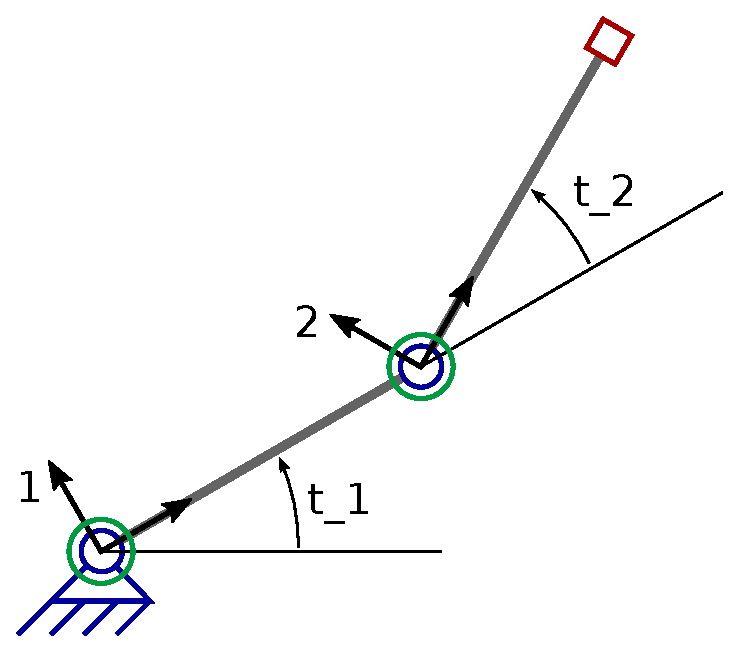
\includegraphics[width=.5\textwidth]{invdyn_2link_fa}
  \caption{Simple example of an inverse dynamics problem: a planar 2-link robot.}
  \label{fig:PROBLEMS:INVDYN:2link_fa}
\end{figure}
With reference to figure~\ref{fig:PROBLEMS:INVDYN:2link}, consider the simple example of a
planar 2-link robot\ldots
\begin{figure}[htbp]
  \centering
  \psfrag{1}{1}
  \psfrag{2}{2}
  \psfrag{t_1}{$\theta_1$}
  \psfrag{t_2}{$\theta_2$}
  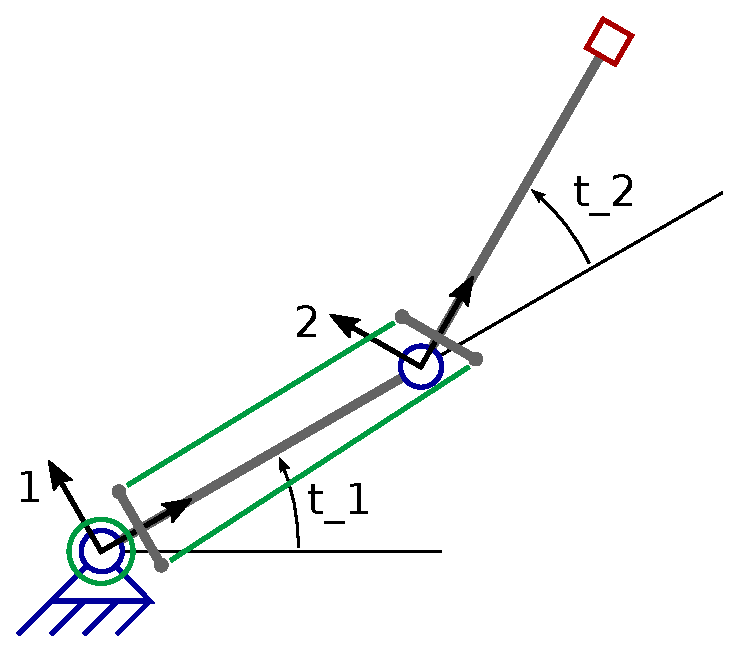
\includegraphics[width=.5\textwidth]{invdyn_2link_oa}
  \caption{Simple example of a kinematically fully determined but overactuated inverse
    dynamics problem: a planar 2-link robot controlled by three actuators.}
  \label{fig:PROBLEMS:INVDYN:2link_oa}
\end{figure}

\begin{figure}[htbp]
  \centering
  \psfrag{1}{1}
  \psfrag{2}{2}
  \psfrag{3}{3}
  \psfrag{t_1}{$\theta_1$}
  \psfrag{t_2}{$\theta_2$}
  \psfrag{t_3}{$\theta_3$}
  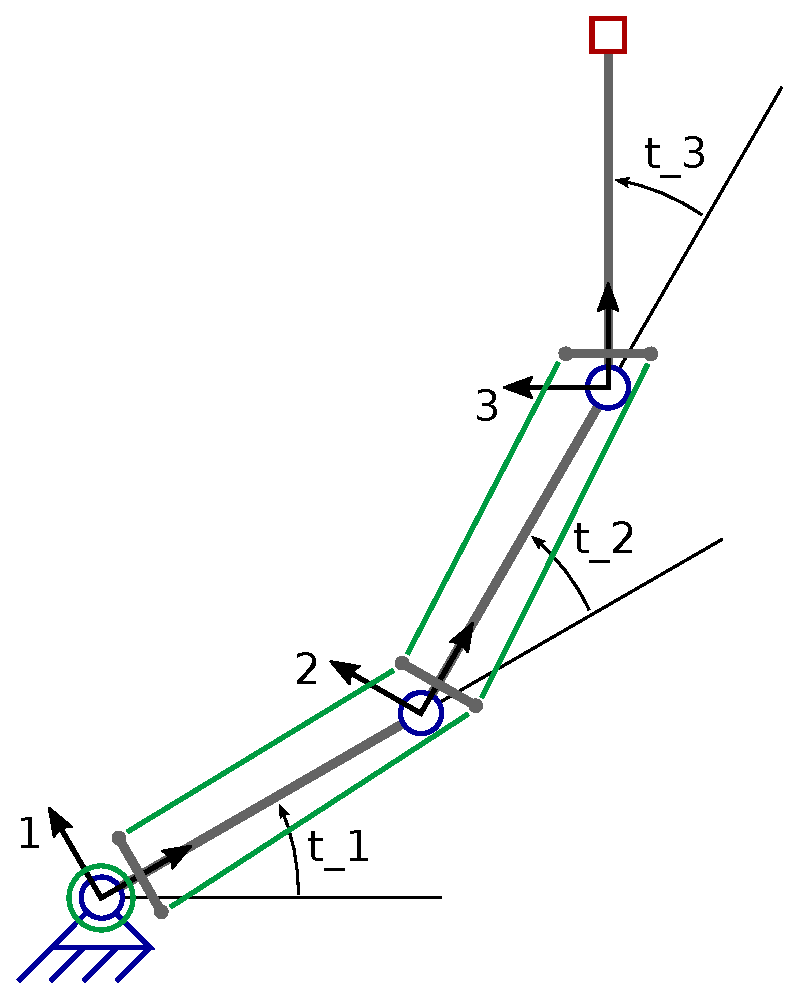
\includegraphics[width=.5\textwidth]{invdyn_3link_oa}
  \caption{Simple example of a kinematically underdetermined, overactuated inverse
  dynamics problem: a planar 3-link robot controlled by five actuators.}
  \label{fig:PROBLEMS:INVDYN:3link_oa}
\end{figure}
% \section{Other Problems}
% Other types of problems are either possible or being developed.
% Typically, static problems can be obtained in terms of a downgrading
% of the initial value problem, by eliminating time-dependent
% interactions and treating time as an ordering parameter.
% 
% A special problem that is currently under development
% is \kw{inverse dynamics}.
